\chapter{Methodology for the placement}

Modern analog automation tools are able to generate analog layout respecting various placement constraints and they mainly use simulated annealing approach. Nevertheless, such approach might not produce predictable and easy-to-adjust results. We believe that giving more control to the designer will generate analog layout, easier to predict compared to optimization-based approach, but also easier to adjust in case modifications are required. Our analog/mixed-signal placer is semi-automatic: the device generation is automated and generated correct-by-construction and guided by the designer's constraints over the circuit. The following sections will describe the interventions from the designer.

\begin{figure}[h]
\begin{center}
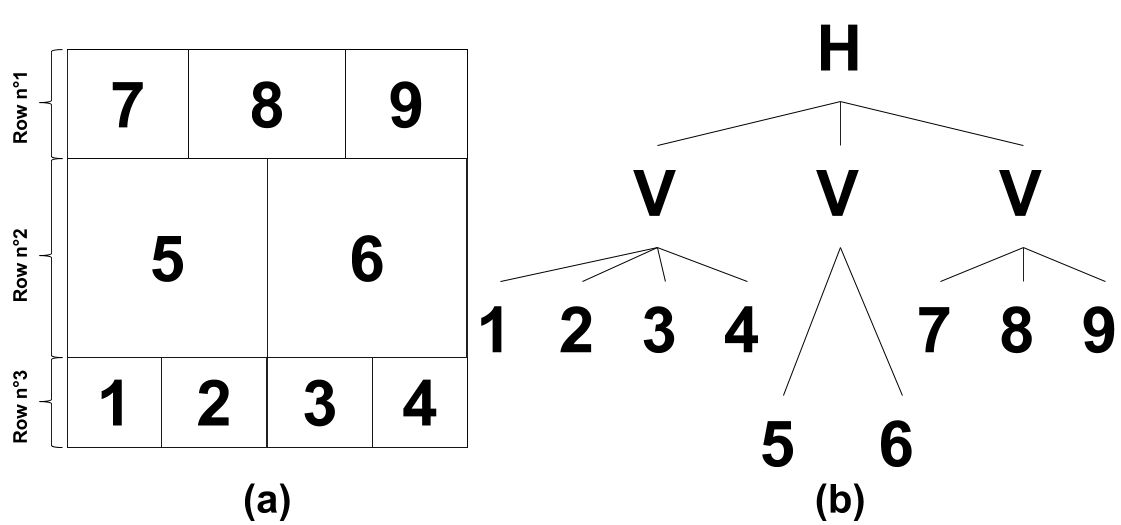
\includegraphics[height=50mm]{Figures/1.png}
caption{Example of placement (a) and its slicing tree representation (b) where "H" stands for horizontal cut and "V" for vertical cut}
\end{center}
\end{figure}
\vspace{-1cm}
\section{Slicing Tree Construction}
In order to organize devices in row, we use the slicing tree structure (Fig. 3) which will be described by the designer and not automatically generated by the placer. Our placer will only assist the designer so it generates the slicing tree according to the designer's constraints. A slicing tree is a slicing floorplan that represents an area that has been divided multiple times either vertically or horizontally, forming a set of rectangular regions representing the place filled by each device. These slices are organized hierarchically so they form a graph where the hierarchical node are either horizontal or vertical cuts. Fig. 3 shows an example of a slicing tree representing a circuit of 9 devices organized in three rows.

\section{Devices Variations}
Our placement approach consists in organizing devices in row, that is to say to have rows of devices with similar height, and the overall analog part's height would be a multiple of standard cell's heights from the digital circuit part. To obtain a row of devices, the height of each device needs to be similar and this is the reason why, we need to consider several possible aspect ratios for each device by varying the number of fingers (Fig. 4) like in cite{6} so we can find heights of devices that match a given height. 
\newline 
\newline 
\indent However varying the number of fingers of a MOS transistor implies a variation of the source/drain capacitance $C_{jSB}$ which can impact the circuit performance. This variation can be calculated using the formula \eqref{1}:

\begin{figure}
  \begin{minipage}[c]{.48\linewidth}
    \begin{center}
      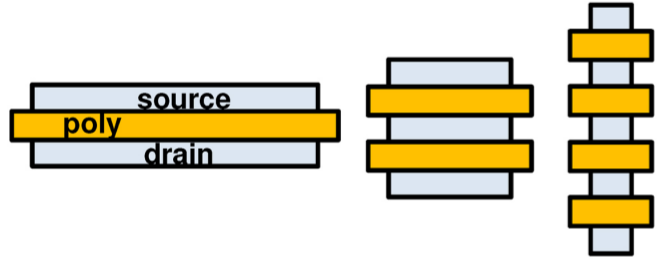
\includegraphics[width=80mm]{Figures/5.png}
      caption{MOS transistor with different finger numbers resulting in different physical dimensions}
    \end{center}
  \end{minipage} \hfill
  \begin{minipage}[c]{.48\linewidth}
    \begin{center}
      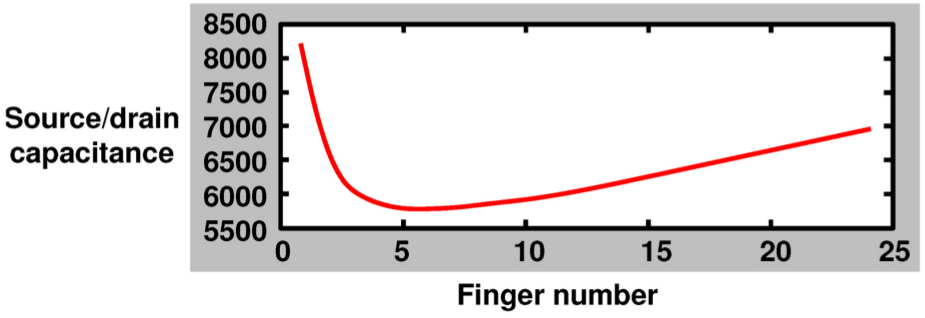
\includegraphics[width=80mm]{Figures/4.png}
      caption{Induced source/drain capacitance of a MOS transistor function cite{6}}
    \end{center}
  \end{minipage}
\end{figure}

\begin{equation}\label{1}
C_{jSB} = \frac{A.C_j}{\Big(1-\frac{V_{BS}}{\phi _j}\Big)^{m_j}}+\frac{P.C_{jsw}}{\Big(1-\frac{V_{BS}}{\phi _j}\Big)^{m_{jsw}}}
\end{equation}
with:
\begin{itemize}
  \setlength\itemsep{0em}
\item $A$ and $P$: source/drain Area and Perimeter
\item $C_j$ and $C_{jsw}$: Bottom and Sidewall junction capacitances 
\item $\phi _j$: built-in junction potential
\item $m_j$ and $m_{jsw}$: depend on the doping profile of the junction
\end{itemize}

Considering a given MOS transistor, its channel width and length is decided by the sizing step and cite{6} presents the following formula of $C_{jSB}$ variation based on the number of fingers:

\vspace{-0.5cm}
\begin{equation}
C_{jSB}(F) = (\alpha .W.L+\alpha .W.\delta _{gap} + 2.\beta .\delta _{gap})+2.\beta .F(L+W.\delta _{gap})+\frac{W}{F} (\alpha .\delta _{gap}+2.\beta)
\end{equation}
with:
\begin{itemize}\label{2}
  \setlength\itemsep{0em}
\item $F$: number of fingers
\item $W$ and $L$: channel Width and Length
\item $\alpha = \Big(1-\frac{V_{BS}}{\phi _j}\Big)^{m_j}$
\item $\beta = \Big(1-\frac{V_{BS}}{\phi _j}\Big)^{m_{jsw}}$
\item $\delta _{gap}$: gap seperating 2 fingers 
\end{itemize}

As cite{2} mentioned, changing the number of fingers of a device can considerably change the source/drain bulk capacitance (Fig. 5) and therefore the device properties. Nevertheless, as mentioned in section 4.1, our placement phase is part of an internal loop, which is repeated until a result meets the required performances (Fig. 2). Also, it is the task of the designer to decide the admissible range of shapes for every device which would limit the number of finger variations.

\section{Margin Tolerances}
We aim at creating rows and it is important to define what we consider as a row of devices. We introduce a tolerance margin, which represents the difference between the smallest and the tallest device's height in a vertical node. Fig. 6 (a) shows an example of devices organized in row where the area A, B, C and D represent devices. Devices A and B show respectively the smallest and highest height inside the row. This difference of height is compared to the tolerance parameter to establish if this is considered as a legal row. We apply the same concept to the horizontal node but instead of using the height as a comparison, we use the width. It is up to the designer to adjust this tolerance margin and it will impact on the number of accepted possibilities. Different margin tolerances can be considered at each hierarchical nodes. At the same time, having a small tolerance will reduce the waste of space induced by the slicing tree representation.

\begin{figure}[h]
\begin{center}
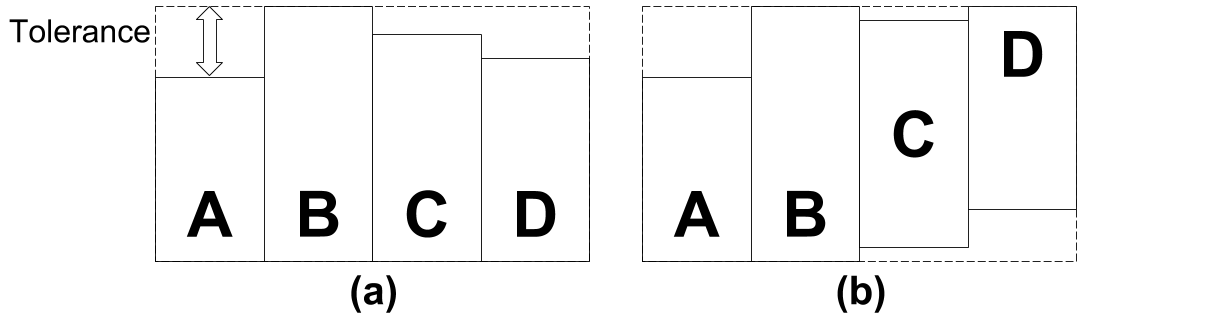
\includegraphics[height=30mm]{Figures/2.png}
caption{Tolerance (a) and alignment (b) in slicing tree representation}
\end{center}
\end{figure}
\vspace{-1cm}
\section{Placement Constraints}
As said in section 3.1, it is the task of the designer to describe the slicing tree with the help of our placer. This will directly impact on the topology of the circuit. This means he will have the total control over the relative relation between the blocks. Having the designer building his own slicing tree also means that he will have control over placement constraints such as proximity, boundary, current/signal path and regularity constraints based on his knowledge and preference.
\newline 
\newline 
\indent Among the most common constraints, symmetries can be respected with the appropriate slicing tree organization. We also consider alignment constraints inside of a slicing tree in horizontal or vertical node. In Fig. 6 (b), we have an example of possible alignments: devices A and B are aligned to the bottom of the row, device C is centered and device D is aligned to the top of the row. In horizontal slices, devices can be aligned to the right, center and left of the row.

\section{Placement Choice}
Similar to cite{17}, once all the possible variations are set for each device, we evaluate the accepted variations at hierarchical nodes based on the margin tolerances. These accepted variations are propagated from the bottom of the slicing tree to the root. After this bottom-up propagation, the designer processes the different placements based on height, width or global ratio criteria. He can choose the most optimized placements according to the Pareto front curve like in cite{18}, but he is free to choose any other possible placement that would eventually have more white space if the circuit can afford more space.